\documentclass[xcolor=dvipsnames,professionalfonts,smaller,presentation]{beamer} 
\usecolortheme[named=Brown]{structure} 
\useoutertheme{miniframes}
\usetheme{Malmoe}
\usepackage{graphicx}
\usepackage{verbatim}
\usepackage[portuguese]{babel}
\usepackage[latin1]{inputenc}
\usepackage{alltt}
\usepackage{moreverb}
\usepackage{hyperref}
\usepackage{indentfirst}
\usepackage{lastpage}
\usepackage{url}
\usepackage{float}
\usepackage{subfigure}

\urldef{\mails}\path|ei05011@fe.up.pt,ei05028@fe.up.pt|
\title[A comparison of classification algorithms applied to the Adult Database \insertframenumber/\inserttotalframenumber]{A comparison of classification algorithms applied to the Adult Database}
\author{Fl�vio Cruz and Jo�o Azevedo}
\institute{Faculdade de Engenharia da Universidade do Porto\\
\mails}
\date{\today}

\begin{document}

\frame{\titlepage}

\section[Outline]{}
\frame{\tableofcontents}

\section{Problem proposed by the Dataset}
\frame
{
    \frametitle{Problem proposed by the Dataset}

    \begin{itemize}
    \item<1-> Given an adult with some attributes, identify whether he gains more than 50000 dollars per year, or not.
    \item<1-> Identify what social characteristics allow one person to gain more than someone else.
    \item<1-> Understanding what affects the income can give a lot of information concerning society's behaviour.
    \end{itemize}
}

\section{Dataset Characterization}

\subsection{The Dataset}
\frame
{
    \frametitle{The Dataset}
    
    \begin{itemize}
    \item<1-> 48842 entries of individual information of people gathered in a 1994 census on the United States of America.
    \begin{itemize}
        \item<1-> 32561 records for the training set (67\%).
        \item<1-> 16281 records for the test set (33\%).
    \end{itemize}
    \item<1-> Each entry is composed by a set of 14 attributes and 2 classes (winning more or less than 50K dollars a year).
    \item<1-> There are 3620 records with missing values. The only attributes containing missing values are \textbf{Workclass}, \textbf{Occupation} and \textbf{Native-country}.
    \item<1-> Available in \url{ftp://ftp.ics.uci.edu/pub/machine-learning-databases/adult}.
    \end{itemize}
}

\frame
{
    \frametitle{Attributes}

    \begin{itemize}
        \item<1-> \textbf{Age} (continuous).
        \item<1-> \textbf{Workclass} (categorical).
        \item<1-> \textbf{FNLWGT} (continuous).
        \item<1-> \textbf{Education} (ordinal).
        \item<1-> \textbf{Education-num} (continuous).
        \item<1-> \textbf{Marital-status} (categorical).
        \item<1-> \textbf{Occupation} (categorical).
        \item<1-> \textbf{Relationship} (categorical).
        \item<1-> \textbf{Race} (categorical).
        \item<1-> \textbf{Sex} (categorical).
        \item<1-> \textbf{Capital-gain} (continuous).
        \item<1-> \textbf{Capital-loss} (continuous).
        \item<1-> \textbf{Hours-per-week} (continuous).
        \item<1-> \textbf{Native country} (categorical).
    \end{itemize}   
}

\subsection{Data Analysis}
\frame
{
    \frametitle{Value distribution in the training set}

\footnotesize
\begin{table}
\subtable[Age]{
       \begin{tabular}{| l | l |}
       \hline
       Min. & 17 \\
       \hline
       1st Qu. & 28 \\
       \hline
       Median & 37 \\
       \hline
       Mean & 38.58 \\
       \hline
       3rd Qu. & 48 \\
       \hline
       Max & 90 \\
       \hline
       \end{tabular}
}
\qquad\qquad
\subtable[Workclass]{        
       \begin{tabular}{| l | l |}
       \hline
       private & 22696 \\
       \hline
       self\_emp\_not\_inc & 2541 \\
       \hline
       local\_gov & 2093 \\
       \hline
       state\_gov & 1298 \\
       \hline
       self\_emp\_inc & 1116 \\
       \hline
       (Other) & 981 \\
       \hline
       NA's & 1836 \\
       \hline
       \end{tabular}
}
\qquad\qquad
\subtable[Education]{        
       \begin{tabular}{| l | l |}
       \hline
       hs\_grad & 10501 \\
       \hline
       some\_college & 7291 \\
       \hline
       bachelors & 5535 \\
       \hline
       masters & 1723 \\
       \hline
       assoc\_voc & 1382 \\
       \hline
       11th & 1175 \\
       \hline
       (Other) & 5134 \\
       \hline
       \end{tabular}
}
\qquad\qquad
\subtable[Marital Status]{        
       \begin{tabular}{| l | l |}
       \hline
       divorced & 4443 \\
       \hline
       married\_af\_spouse & 23 \\
       \hline
       married\_civ\_spouse & 14976 \\
       \hline
       married\_spouse\_absent & 418 \\
       \hline
       never\_married & 10683 \\
       \hline
       separated & 1025 \\
       \hline
       widowed & 993 \\
       \hline
       \end{tabular}
}
\end{table}
\normalsize
}

\frame
{
    \frametitle{Value distribution in the training set}

\footnotesize
\begin{table}
\subtable[Occupation]{        
       \begin{tabular}{| l | l |}
       \hline
       prof\_specialty & 4140 \\
       \hline
       craft\_repair & 4099 \\
       \hline
       exec\_managerial & 4066 \\
       \hline
       adm\_clerical & 3770 \\
       \hline
       sales & 3650 \\
       \hline
       (Other) & 10993 \\
       \hline
       NA's & 1843 \\
       \hline
       \end{tabular}
}
\qquad\qquad
\subtable[Relatonship]{        
       \begin{tabular}{| l | l |}
       \hline
       husband & 13193 \\
       \hline
       not\_in\_family & 8305 \\
       \hline
       other\_relative & 981 \\
       \hline
       own\_child & 5068 \\
       \hline
       unmarried & 3446 \\
       \hline
       wife & 1568 \\
       \hline
       \end{tabular}
}
\qquad\qquad
\subtable[Race]{        
       \begin{tabular}{| l | l |}
       \hline
       amer\_indian\_eskimo & 311 \\
       \hline
       asian\_pac\_islander & 1039 \\
       \hline
       black & 3124 \\
       \hline
       other & 271 \\
       \hline
       white & 27816 \\
       \hline
       \end{tabular}
}
\qquad\qquad
\subtable[Sex]{        
       \begin{tabular}{| l | l |}
       \hline
       female & 10771 \\
       \hline
       male & 21790 \\
       \hline
       \end{tabular}
}
\end{table}
\normalsize
}

\frame
{
    \frametitle{Value distribution in the training set}

\footnotesize
\begin{table}
\subtable[Capital Gain]{        
       \begin{tabular}{| l | l |}
       \hline
       Min. & 0 \\
       \hline
       1st Qu. & 0 \\
       \hline
       Median & 0 \\
       \hline
       Mean & 1078 \\
       \hline
       3rd Qu. & 0 \\
       \hline
       Max. & 99999 \\
       \hline
       \end{tabular}
}
\qquad\qquad
\subtable[Capital Loss]{        
       \begin{tabular}{| l | l |}
       \hline
       Min. & 0 \\
       \hline
       1st Qu. & 0 \\
       \hline
       Median & 0 \\
       \hline
       Mean & 87.3 \\
       \hline
       3rd Qu. & 0 \\
       \hline
       Max. & 4356 \\
       \hline
       \end{tabular}
}
\qquad\qquad
\subtable[Hours Per Week]{        
       \begin{tabular}{| l | l |}
       \hline
       Min. & 1 \\
       \hline
       1st Qu. & 40 \\
       \hline
       Median & 40 \\
       \hline
       Mean & 40.44 \\
       \hline
       3rd Qu. & 45 \\
       \hline
       Max. & 99 \\
       \hline
       \end{tabular}
}
\qquad\qquad
\subtable[Native Country]{        
       \begin{tabular}{| l | l |}
       \hline
       United States & 29170 \\
       \hline
       Mexico & 643 \\
       \hline
       Philippines & 198 \\
       \hline
       Germany & 137 \\
       \hline
       Canada & 121 \\
       \hline
       (Other) & 1709 \\
       \hline
       NA's & 583 \\
       \hline
       \end{tabular}
}
\qquad\qquad
\subtable[Plus 50]{        
       \begin{tabular}{| l | l |}
       \hline
       No & 24720 \\
       \hline
       Yes & 7841 \\
       \hline
       \end{tabular}
}
\end{table}
\normalsize
}

\frame
{
    \frametitle{Some obvious relationships}
    
    \begin{itemize}
    \item<1-> There is a higher percentage of older people gaining more than 50K than younger ones.
    \item<1-> There is a higher percentage of people with more education gaining more than 50K than people with less studies.
    \item<1-> There is a higher percentage of workaholics gaining more than 50K than people who work in part-time.
    \end{itemize}

   \begin{minipage}{0.30\linewidth}
        \begin{figure}
        \centering
            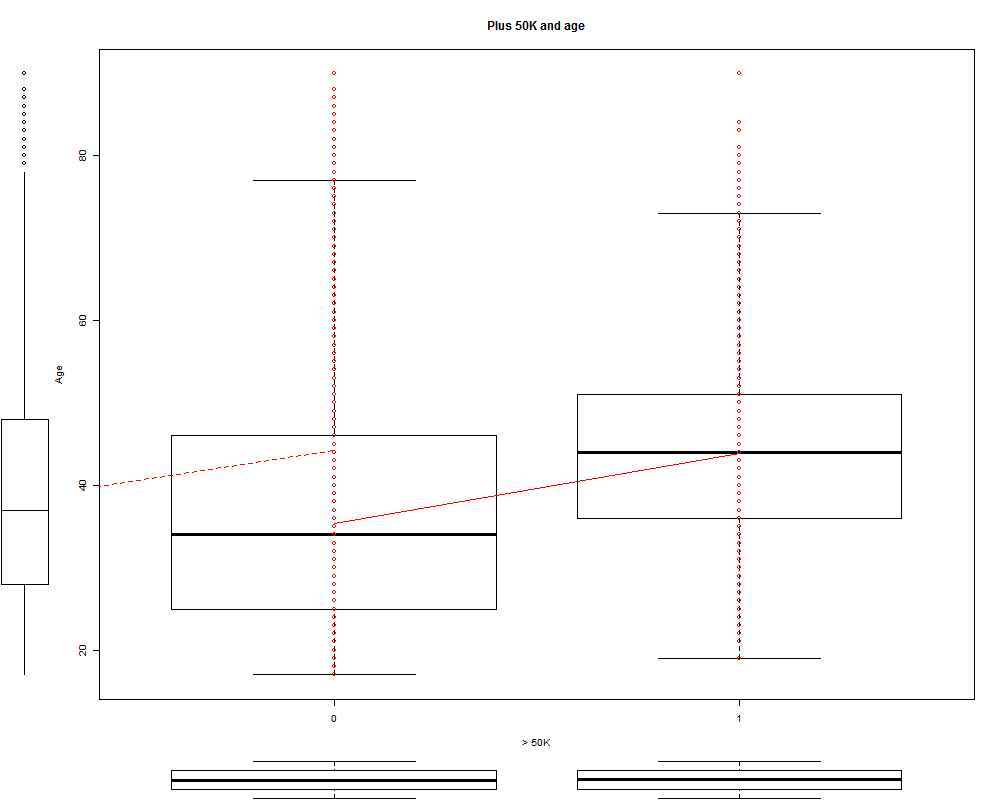
\includegraphics[width=3.5cm]{plot_plus_50_age.png}
        \end{figure}
    \end{minipage}
    \hspace{0.1cm}
    \begin{minipage}{0.30\linewidth}
        \begin{figure}
        \centering
            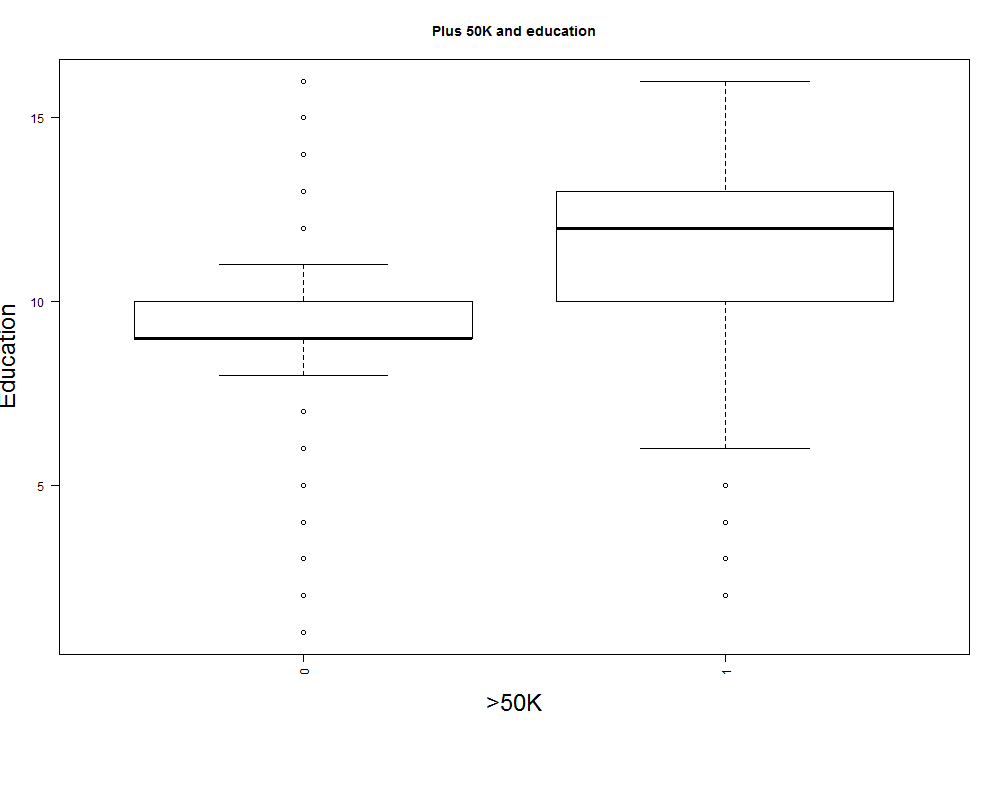
\includegraphics[width=3.5cm]{plot_plus_50_education_num.png}
        \end{figure}
    \end{minipage}
    \hspace{0.1cm}
    \begin{minipage}{0.30\linewidth}
        \begin{figure}
        \centering
            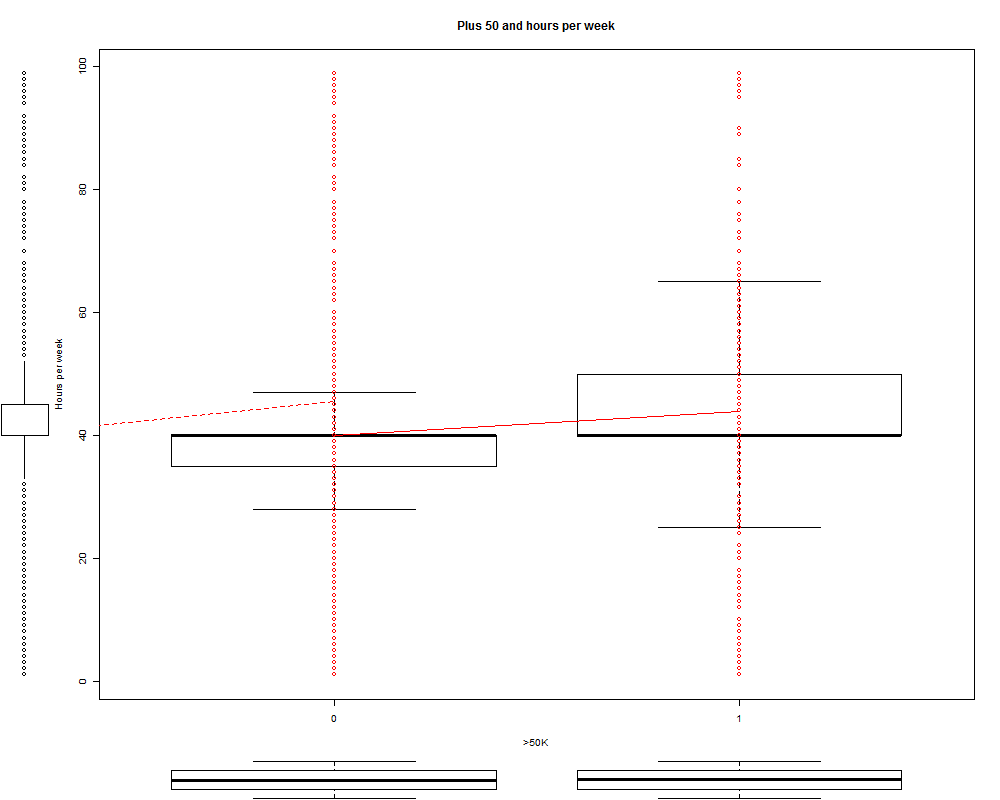
\includegraphics[width=3.5cm]{plot_plus_50_hpw.png}
        \end{figure}
    \end{minipage}
}

\frame
{
    \frametitle{Association Rules}
}

\frame
{
    \frametitle{Clusters}
}

\section{Data Mining Problem}
\frame
{
    \frametitle{Data Mining Problem}

    \begin{itemize}
    \item<1-> The database poses a classification problem.
    \item<1-> There is no single classifier that works best on all given problems:
    \begin{itemize}
        \item<1-> Decision trees.
        \item<1-> Rule induction.
        \item<1-> Inductive logic programming.
        \item<1-> Bayesian classifiers.
    \end{itemize}
    \end{itemize}
}

\section{Algorithms Used}

\subsection{Decision Trees}
\frame
{
}

\subsection{Rule Induction}
\frame
{
}

\subsection{Inductive Logic Programming}
\frame
{
}

\subsection{Bayesian Classifiers}
\frame
{
}

\section{Conducted Experiments}
\frame
{
}

\section{Results}
\frame
{
    \frametitle{Results}

\begin{table}[ht]
    \begin{center}
    \begin{tabular}{ | l | l | l | }
    \hline
    \textbf{Algorithm} & \textbf{Error rate} & \textbf{Time} \\ \hline
    CN2 & 15.20 & 03m29s \\ \hline
    ID3 & 15.68 & 00m14s \\ \hline
    ADTree & 18.49 & 01m12s \\ \hline
    C4.5 & 18.84 & 00m08s \\ \hline
    Bayesian Networks (Simulated Annealing) & 19.15 & 00m07s \\ \hline
    Bayesian Networks (Hill Climbing) & 20.03 & 00m07s \\ \hline
    ILP (Aleph) & 20.45 & $>$ 6hours \\ \hline
    Random Forest & 21.01 & 00m08s \\ \hline
    Bayesian Networks (Genetic Search) & 21.26 & 00m04s \\ \hline
    CART & 21.34 & 07m05s \\ \hline
    \end{tabular}
    \label{tbl:overall_results}
    \end{center}
\end{table}
}

\section{Conclusions}
\frame
{
    \frametitle{Conclusions}

    \begin{itemize}
    \item<1-> ID3 and C4.5 are very fast and build classifiers with a decent error rate.
    \item<1-> ILP and CN2 build more expressive classifiers, capable of a better interpretation by a human agent, but take longer to finish.
    \item<1-> The worst error rate is below 25\%.
    \item<1-> There is a lot of software tools that support the building of classifiers, namely Weka and RapidMiner.
    \begin{itemize}
        \item<1-> Open source.
        \item<1-> Easy to use.
        \item<1-> APIs for integration with Java applications.
    \end{itemize}
    \end{itemize}
}

\frame
{
    \frametitle{Conclusions}

    \begin{itemize}
    \item<1-> Having a high capital gain clearly contributes to gain more than 50K dollars per year.
    \item<1-> Middle-aged husbands have a higher tendency to gain more than 50K dollars per year.
    \item<1-> A high percentage of people who gain less than 50K dollars per year are own childs.
    \item<1-> People coming from countries such as Taiwan, Thailand or Cambodia usually have higher education and gain more than 50K dollars per year.
    \end{itemize}
}

\end{document}
